\section[Swiss E-Government]{Swiss E-Government (CH e-Gov)}
\label{main}
This report is focused on eGovernment, but what is e-government?\\
E-government (short for electronic government) is the use of technologies (computers, internet, databases, etc.) for public administration in order to unite the highest parts of government with local authorities.
In this way the government and everything around it can provide itself as a service to the citizen.
The citizen will then be able to use this service in a simpler, faster way without having to go to the authorities in person.\\

Before analyzing how an eGovernment is structured we have to ask ourselves if it makes sense to have an eGovernment, analyzing the pros and cons.

\begin{longtable}[ c ]{|l|l|}
\hline
\multicolumn{2}{| c |}{\textbf{Pros and Cons eGovernment}}   \\ \hline
\endfirsthead
%
\multicolumn{2}{c}%
{{\bfseries Table \thetable\ continued from previous page}} \\
\hline
\multicolumn{2}{| c |}{\textbf{Pros and Cons eGovernment}}   \\ \hline
\endhead
%
\textbf{Pros}             & \textbf{Cons}                  \\ \hline
Data accuracy             & Expensive IT system            \\ \hline
Access to data            & All IT-related problems        \\ \hline
Ease of Data Verification & Security and terrorist attacks \\ \hline
Ease of Data Updates      & Dependence on electricity      \\ \hline
Ease of Data Archiving    & Network issues                 \\ \hline
\caption{Pros and Cons eGovernment}
\label{tab:eGovProCons}\\
\end{longtable}

From the table it can be understood that in the face of the obvious pros, there are also some very important cons.
For this reason, governments around the world, as they move to digital, create strategies to improve themselves over time, thereby reducing the list of cons.\\

\subsection[Project architecture]{Project architecture (statics)}
To better understand the government we must first know the story.\\
The Swiss Confederation was re-established as a result of the Act of Mediation issued by Napoleon Bonaparte on 19 February 1803.\\
In the opening letter of the first meeting Napoleon wrote to the Swiss delegates:

\epigraph{“\textit{Switzerland does not resemble any other country in terms of the events that have taken place there over the centuries, its geographical and topographical situation, its different languages and religious denominations, and the extreme difference in customs that exists between its different parts. Nature has made your country a federal state: it is not wise to want to win it.}”}{}

Switzerland is a federal state, which means that state power is divided between the Confederation, the 26 cantons and about 2300 municipalities.  \\
Federalism allows the 3 levels of the state to have their own political competences, and that local authorities have the highest possible autonomy.\\

%\begin{figure}[!htb]
\begin{figure}[H]
\centering
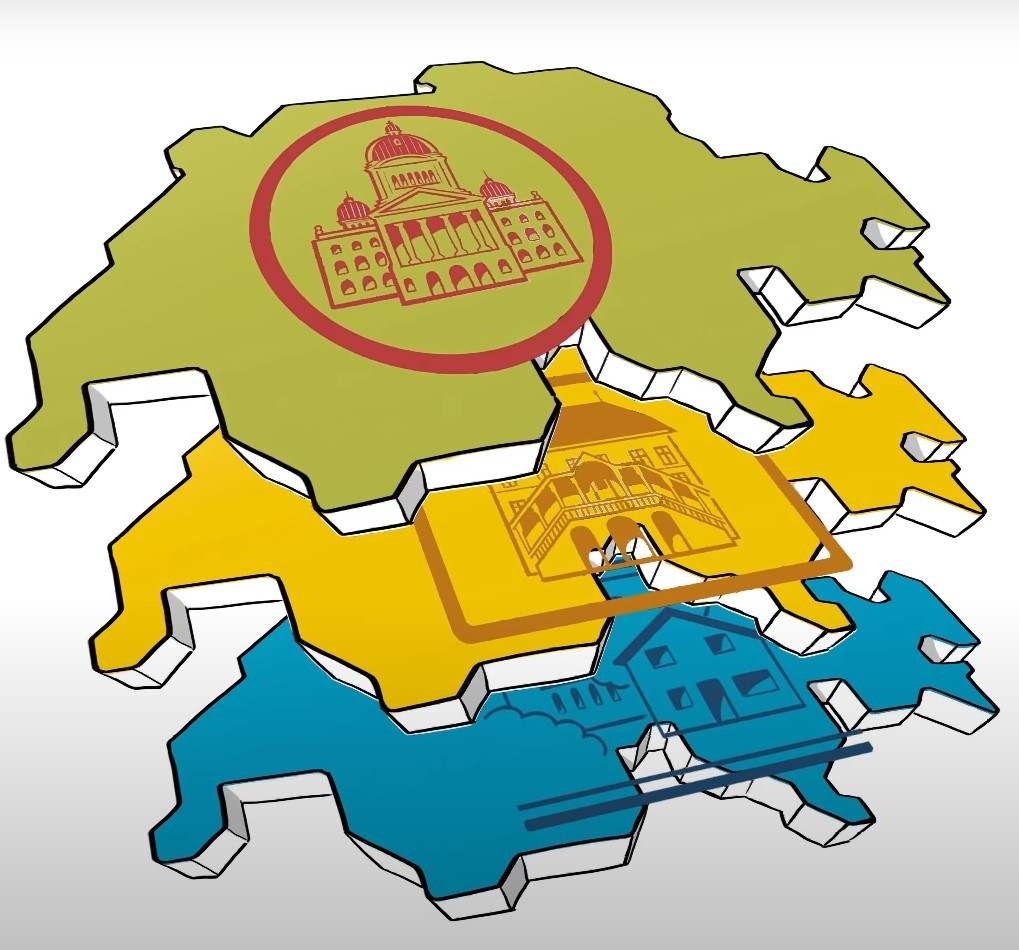
\includegraphics[scale=0.25]{images/trepoteri.jpg}
\caption{The 3 level}
\label{fig:file_3pow}
\end{figure}
%\FloatBarrier

The Confederation therefore only assumes tasks which are beyond the capabilities of the cantons, as well as the cantons to the municipalities.
However, citizens have the last word at all 3 state levels, thanks to direct democracy.

\subsubsection{Confederation}
The Confederation is competent in the areas in which the Federal Constitution authorizes it to be. In particular in the following areas:
\begin{itemize}
\item foreign policy and security;
\item border and monetary policy;
\item legislation valid at national level;
\item protection.
\end{itemize}

The confederation has over time created several digital portals, in order to group all the data concerning the government. In doing so it has become easier for citizens and other authorities to consult information, but also to receive notices, announcements from the confederation. The main portals are:
\begin{itemize}
\item \url{https://www.admin.ch/}\cite{admin}
\item \url{https://www.ch.ch/}\cite{chch}
\item \url{https://www.egovernment.ch/}\cite{egovCH}
\end{itemize}
 
Other smaller portals are also available, but most of them always have a link to "www.admin.ch".\\
The \textit{www.admin.ch} is the main site, with all the information about Switzerland at a macroscopic level, in particular for the digital administration for general public, and also everything that concerns the constitution and bureaucracy.
At \textit{admin.ch} the Federal Chancellery publishes information on the activities and decisions of the Federal Council as well as on federal law. 

%\begin{figure}[!htb]
%\centering
%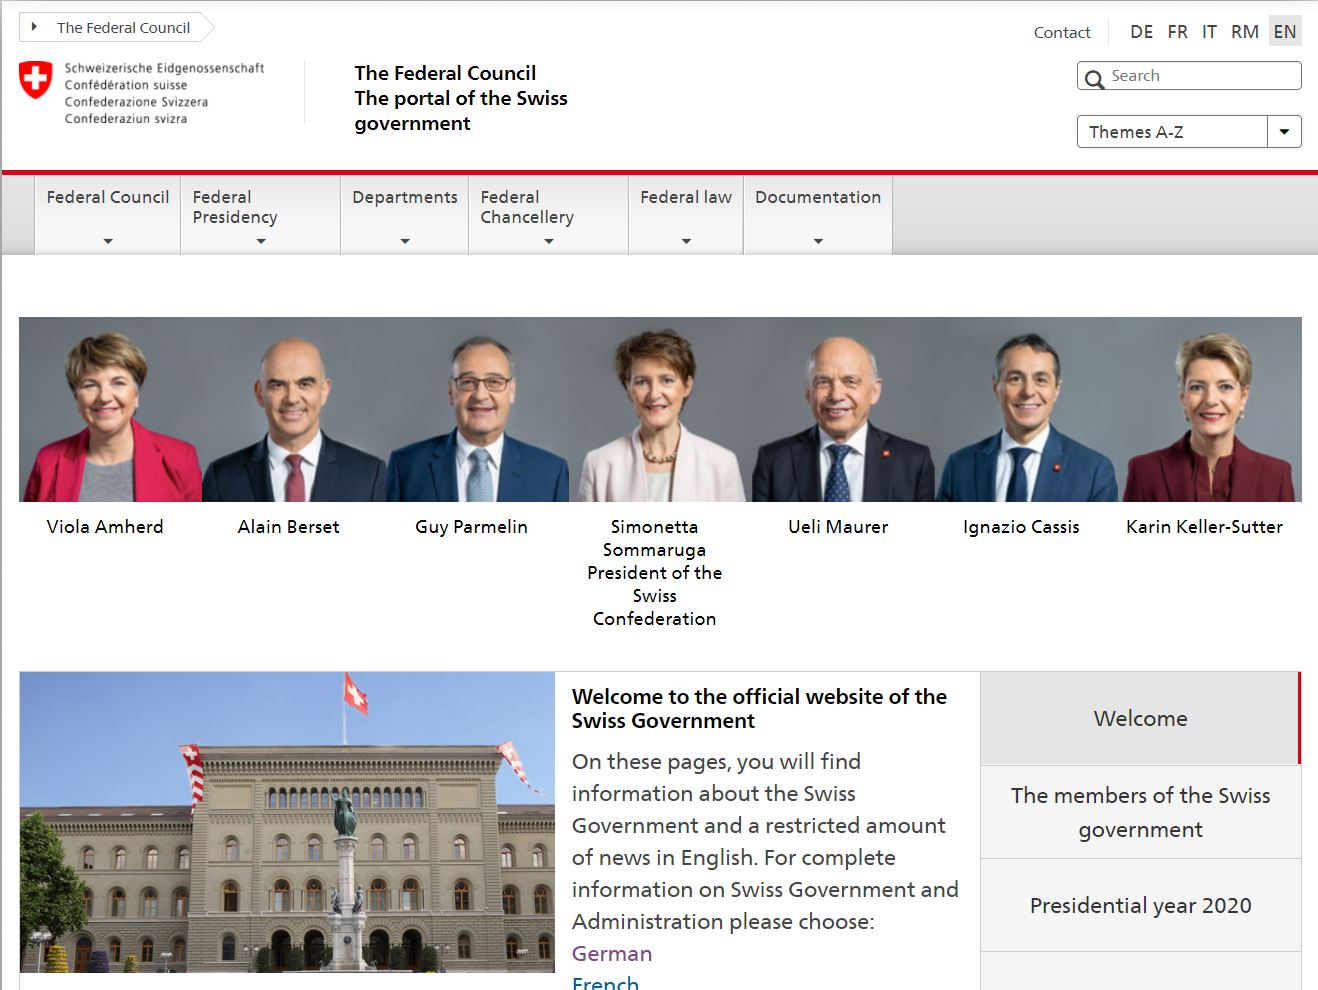
\includegraphics[width=0.5\textwidth]{images/admin.jpg}
%\caption{admin.ch Website \label{overflow}}
%\end{figure}
%\FloatBarrier

If we want to get information or details about individual cantonal or communal information, the site bounces us to specific sites in the cantons or municipalities.\\

As \textit{"admin.ch"} also \textit{"ch.ch"} has a fundamental role in the world of digital governance.
\textit{"ch.ch"} is a user friendly portal (much more than admin), where often the information is reported to the citizen in the form of images, videos, or diagrams easier to understand.
\textit{"ch.ch"} defines itself as \textit{"a rather different Swiss portal for citizens"}. Founded in 2003, it is a collaboration between the three levels of the Swiss government, headed by the Federal Chancellery. It records almost 18 million visits every year, and in addition to social media channels it is translated into 5 languages.

\textit{"egovenrment.ch"} compared to the first two portals, is a portal containing information on the state of e-government.

\subsubsection{Cantons}
Each canton has its own constitution, laws, parliament, government and courts. Every canton deals mainly with:
\begin{itemize}
\item budget
\item the political system
\item taxation
\end{itemize}

The partition that we have in the real world is also found in the digital world, in fact under the level "government" with the sites admin and ch etc., we find the cantonal sites such as \url{https://www.be.ch/}.\\
%\begin{figure}[!htb]
%\centering
%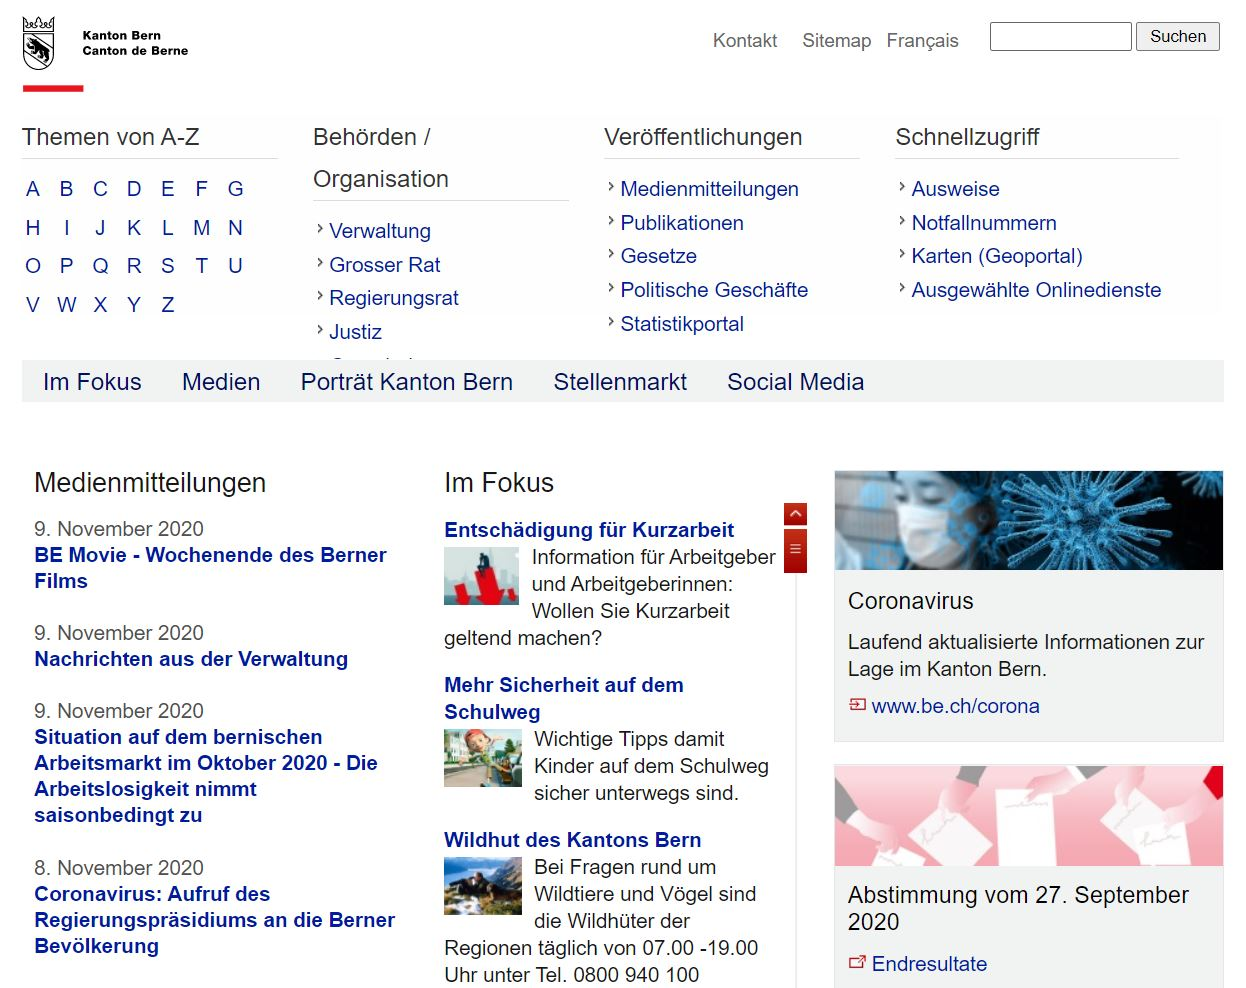
\includegraphics[width=0.5\textwidth]{images/be.jpg}
%\caption{be.ch Website \label{overflow}}
%\end{figure}
%\FloatBarrier

All the information about a single canton can be found, making the information more fragmentary, but also more detailed.
In fact, if a resident is in Canton Bern, he or she will never go looking for information on the Canton Ticino website, making his or her search easier.\\

%Ogni singolo cantone è diverso e quindi anche la regolamentazione è diversa.
On the website of the canton of Bern we can find information about referendums (direct democracy) or information about the city of Bern, the institutions or what the canton itself offers the citizen.

A service of the Canton Bern is the BE-login. With this service you can, for example, fill out fee forms, analyze your data, apply for scholarships or search for information about driving licenses and the similar in a digital way.

%\begin{figure}[!htb]
%\centering
%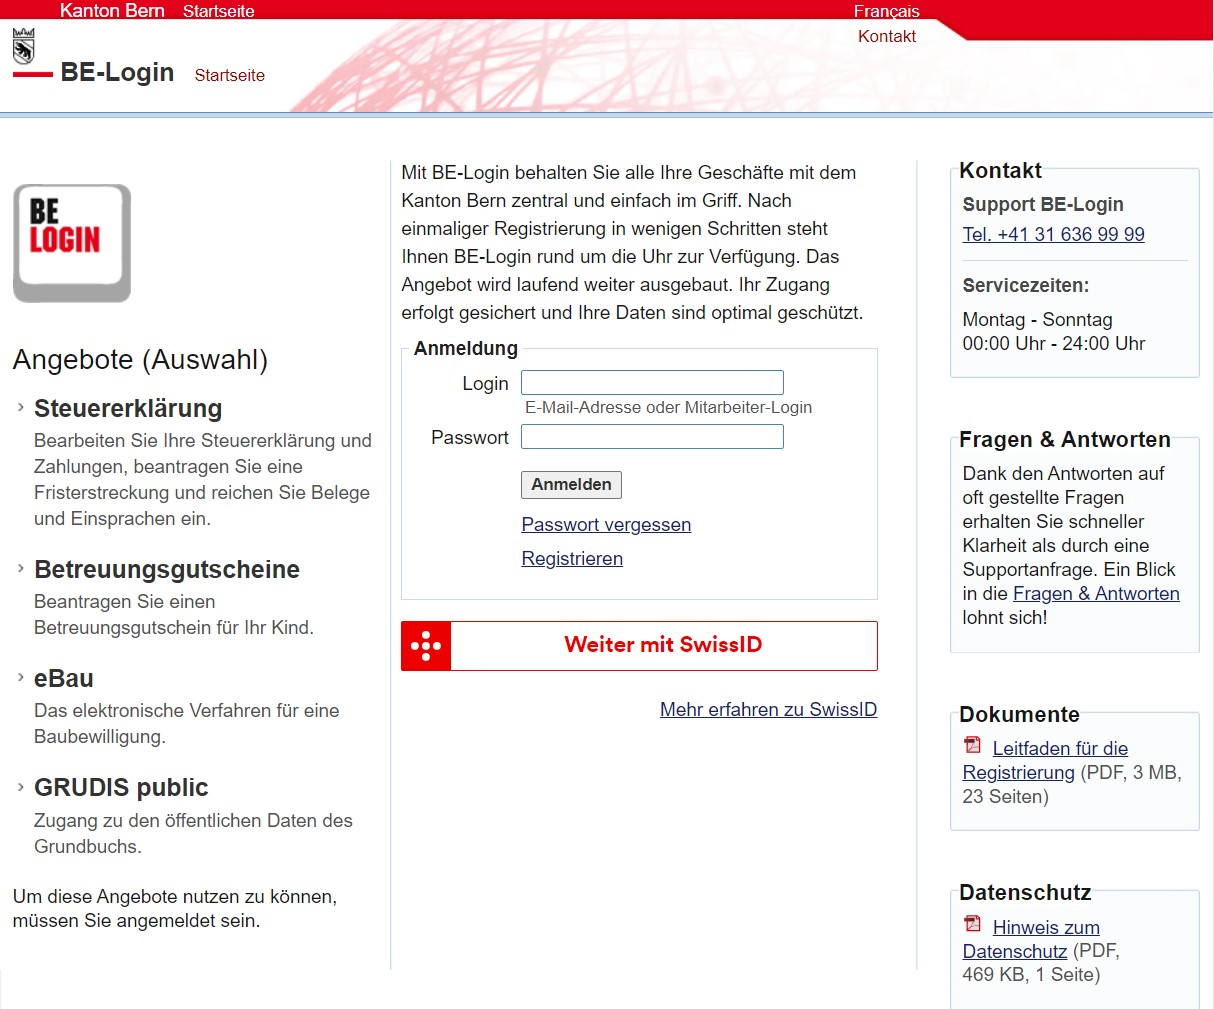
\includegraphics[width=0.5\textwidth]{images/belogin1.jpg}
%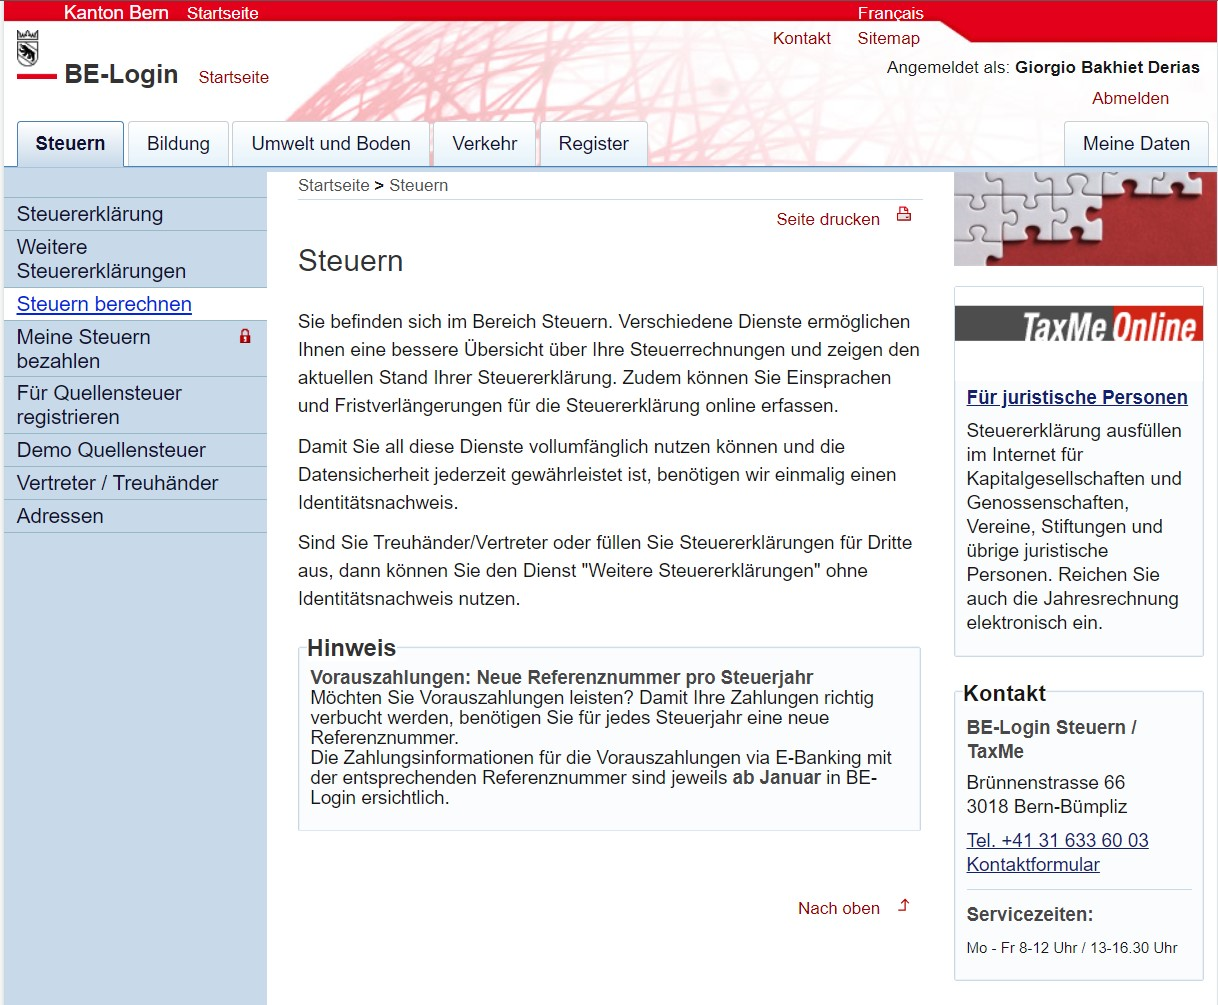
\includegraphics[width=0.5\textwidth]{images/beloginTax.jpg}
%\caption{Be-Login Website \label{overflow}}
%\end{figure}
%\FloatBarrier

\subsubsection{Comunes}
The smallest political unit in Switzerland is the municipality.
Municipalities are mainly concerned with:
\begin{itemize}
\item school and sociality
\item energy supply
\item road construction
\item local planning
\item taxes
\end{itemize}

Most municipalities in Switzerland are small to medium sized, so even the digital part of the individual municipalities is not very advanced.\\
In most cases, the sites are points where you can get information about the territory, opening hours of offices or notices.
%An example of a municipal website we have with the municipality of Kehrsatz, just south of Bern with a population of about 4000 inhabitants. 


%\begin{figure}[!htb]
%\centering
%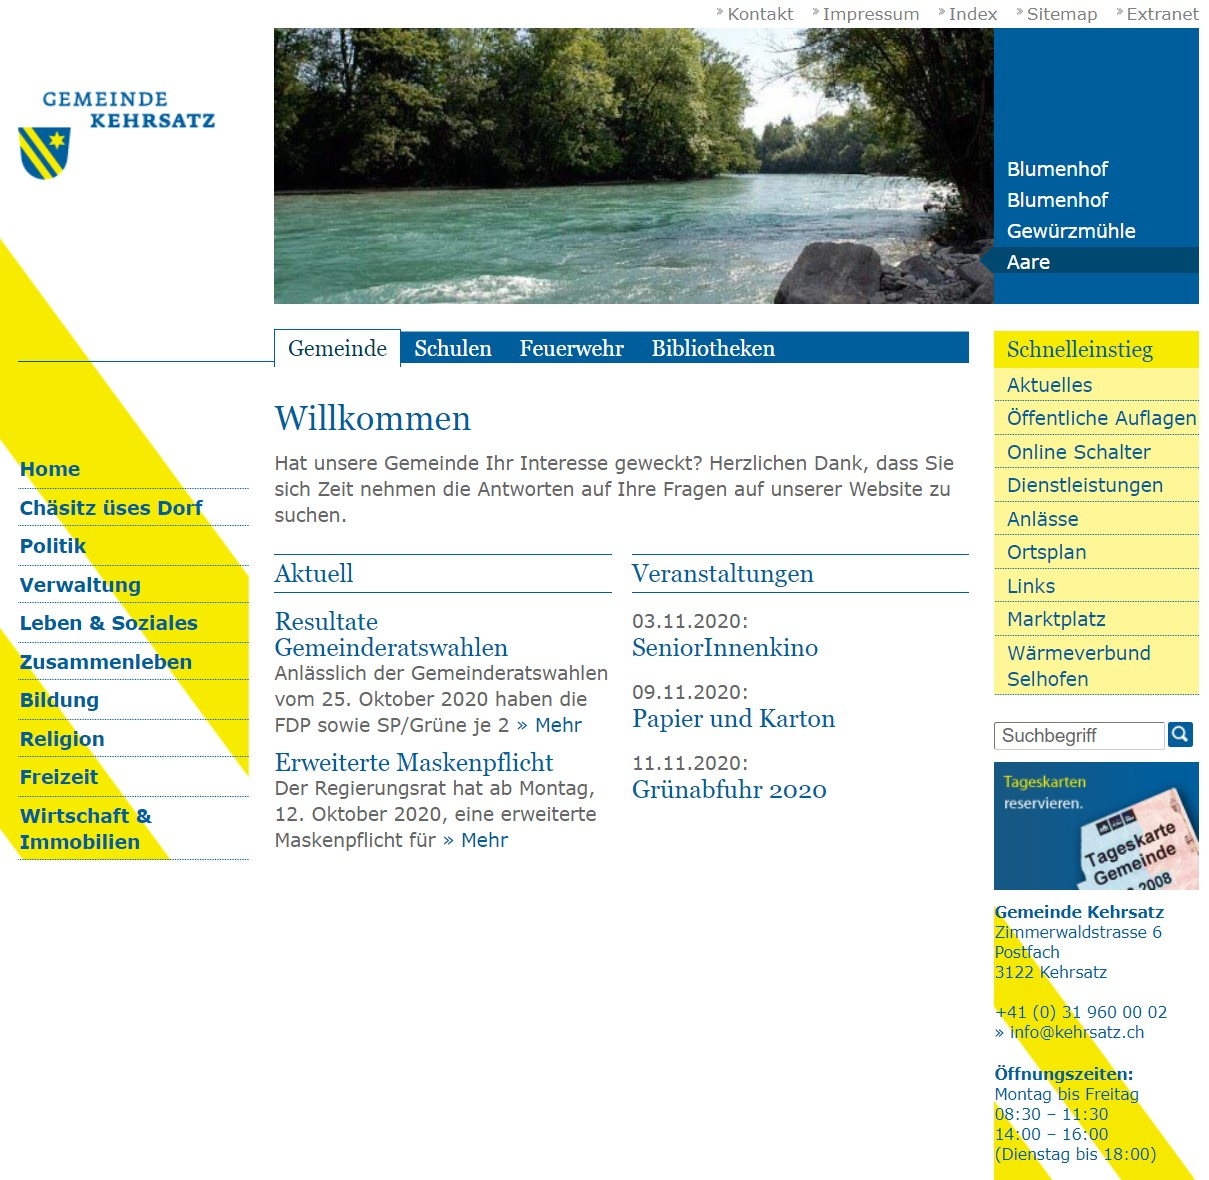
\includegraphics[width=1\textwidth]{images/Kehrsatz.jpg}
%\caption{Kehrsatz Website \label{overflow}}
%\end{figure}
%\FloatBarrier

\subsubsection{One for All}
The Swiss IT Conference founded eOperations Switzerland AG on 20 June 2018.\\
This company simplifies cooperation between the federal government, cantons and municipalities in the field of electronic services for the population and the economy. \\
In this way the procedures for e-government, for the public and businesses, are speeded up and costs reduced, because all solutions come from a single entity.\\
The expansion of eOperations Switzerland is part of the Swiss eGovernment Guidelines for the Confederation and the Cantons.\\

eOperations Switzerland can be consulted at: \url{https://www.eoperations.ch/}\\

The eOperation company plays a key role in the development of eGov in Switzerland,
indeed it develops, proposes to expand and manage shared IT solutions for the authorities.
In this regard, the company has drawn up a list of its services, with the various projects in progress, under discussion and those concluded.\\

\begin{longtable}[ c ]{| m{4cm} | m{9.5cm}|}
\hline
\multicolumn{2}{| c |}{\textbf{Projects in progress}}                                                                                                                                                      \\ \hline
\textbf{Project} & \textbf{Description                                                                                                } \\ \hline
\endfirsthead

\multicolumn{2}{c}
{{\bfseries Table \thetable\ continued from previous page}} \\
\hline
\textbf{Project} & \textbf{Description} \\ \hline
\endhead

eMovingCH & Electronic notification of change of residence. In January 2018 the management of the service was assigned to eOperations Switzerland in order to make  it available to the other cantons that had expressed  interest.\\ \hline
Digital document \newline signature validation system & The signature validation system can be used to verify if the electronic documents are validly signed. In the future, the solution will be available not only to the Confederation, but also to the cantons and municipalities interested. The productive use of this project will be for mid 2021.\\ \hline
Acquisition of\newline "standard telecommunications serivices" & The Swiss Conference on Information Technology charges eOperations Switzerland to manage the project to reduce the costs of standard telecommunications services for Swiss administrations. \\ \hline
Long life time digital archiving & This project is still under discussion between people specialized in archives of various municipalities and eOperations Switzerland. \\ \hline
\acrlong{ins} & \acrshort{ins} simplifies access to electronic services for citizens, businesses and even government employees. It allows digital collaboration between all authorities that are involved.\\ \hline
1st level helpdesk\newline organization for \newline municipalities & Outsource the support of the municipalities, such as the eMovingCH service. \\ \hline
\caption{eOperations project in progress}
\label{eOpProgress}\\
\end{longtable}

\begin{table}[h!]
\centering
%\resizebox{\textwidth}{!}{%
\begin{tabular}[ c ]{| m{2.5cm} | m{11cm}|}
\hline
\multicolumn{2}{|c|}{\textbf{Projects under discussion}}                                                                                                                                                                                                                                                                                \\ \hline
\textbf{Project} & \textbf{Description}                                                                                                                                                                                                                                                                                                                \\ \hline
Publibrain & \begin{tabular}[c]{@{}l@{}}TheThe goal is to make knowledge at the administrative level \\ available to those who need it.\\ For this purpose, the project connects people from various \\ administrative organizations and their know-how.\\ Machine learning and user friendly graphics make it easy to use\end{tabular} \\ \hline
\end{tabular}%
%}
\caption{eOperations under discussion projects}
\label{eOpDiscussion}
\end{table}


\begin{table}[h!]
\centering
%\resizebox{\textwidth}{!}{%
\begin{tabular}[ c ]{| m{3.5cm} | m{10cm}|}
\hline
\multicolumn{2}{|c|}{\textbf{Concluded projects}}                                                                                                                                                                                                                                                            \\ \hline
\textbf{Project}                                                                                   & \textbf{Description}                                                                                                                                                                                                      \\ \hline
\begin{tabular}[c]{@{}l@{}}Development and \\ management \\ of eCH standards\end{tabular} & \begin{tabular}[c]{@{}l@{}}eOperations Switzerland acquires, through a public tender, \\ services for the development of \acrshort{xml} standards for the \\ building registration and notification procedure.\end{tabular} \\ \hline
\end{tabular}%
%}
\caption{eOperations concluded projects}
\label{eOpFinish}
\end{table}

Source listed projects: \cite{eOPProj}
\newpage

\subsection[Project evolution]{Project evolution (dynamics)}
In this section we can see how e-gov has evolved dynamically by analyzing the three phases: past, present and future.

\subsubsection{eGovernment History}
Since 2008, the Confederation, cantons and municipalities have been working together to create the eGovernment. For this reason, they have defined various strategies together, and a \href{https://www.egovernment.ch/en/organisation/steuerungsausschuss/}{\emph{Swiss e-government organization}} has been created to implement these strategies.\\
Besides this organization, there are other organizations that promote the use of information technology and the use of digital administration, such as \href{https://sik.swiss/}{\emph{the Swiss IT conference "\acrshort{sik}/CSI"}} and also \href{https://www.egovernment.ch/en/organisation/projekt-und-leistungsverantwortliche/verein-ech/}{\emph{the Swiss standardization association "eCH"}}.\\

\textbf{Youth problems} in fact it is only 2007 when:
\begin{quote}Switzerland was ranked 26th out of 31 European countries for the sophistication and availability of its online public services.

The report found that only 21\% of the monitored public services were fully available online in Switzerland – up 10\% on 2006 - compared with the European average of 58\%.~\cite{swisslags2007}\end{quote}

The situation starts to move only in 2018, in fact it is established:
\begin{itemize}
\item egovernment.ch
\item eoperations.ch
\item e-voting has been introduced
\item e-ID
\end{itemize}

which is not enough, in fact, Switzerland is still among the last of the 34 European countries.\\

Was conducted by a German research group, an e-gov survey to find out how many Swiss are using electronic services unfortunately what was found was:
\begin{quotation}
"the proportion of the Swiss population using e-government services had fallen from 58\% in 2012 to 55\% in 2018."\cite{swisslags}
\end{quotation}

\newpage
Figure 2, just below, describes the use of eGovernment from 2012 to 2020 by citizens ranges from 58\% to 60\%.

\begin{figure}[!htb]
\centering
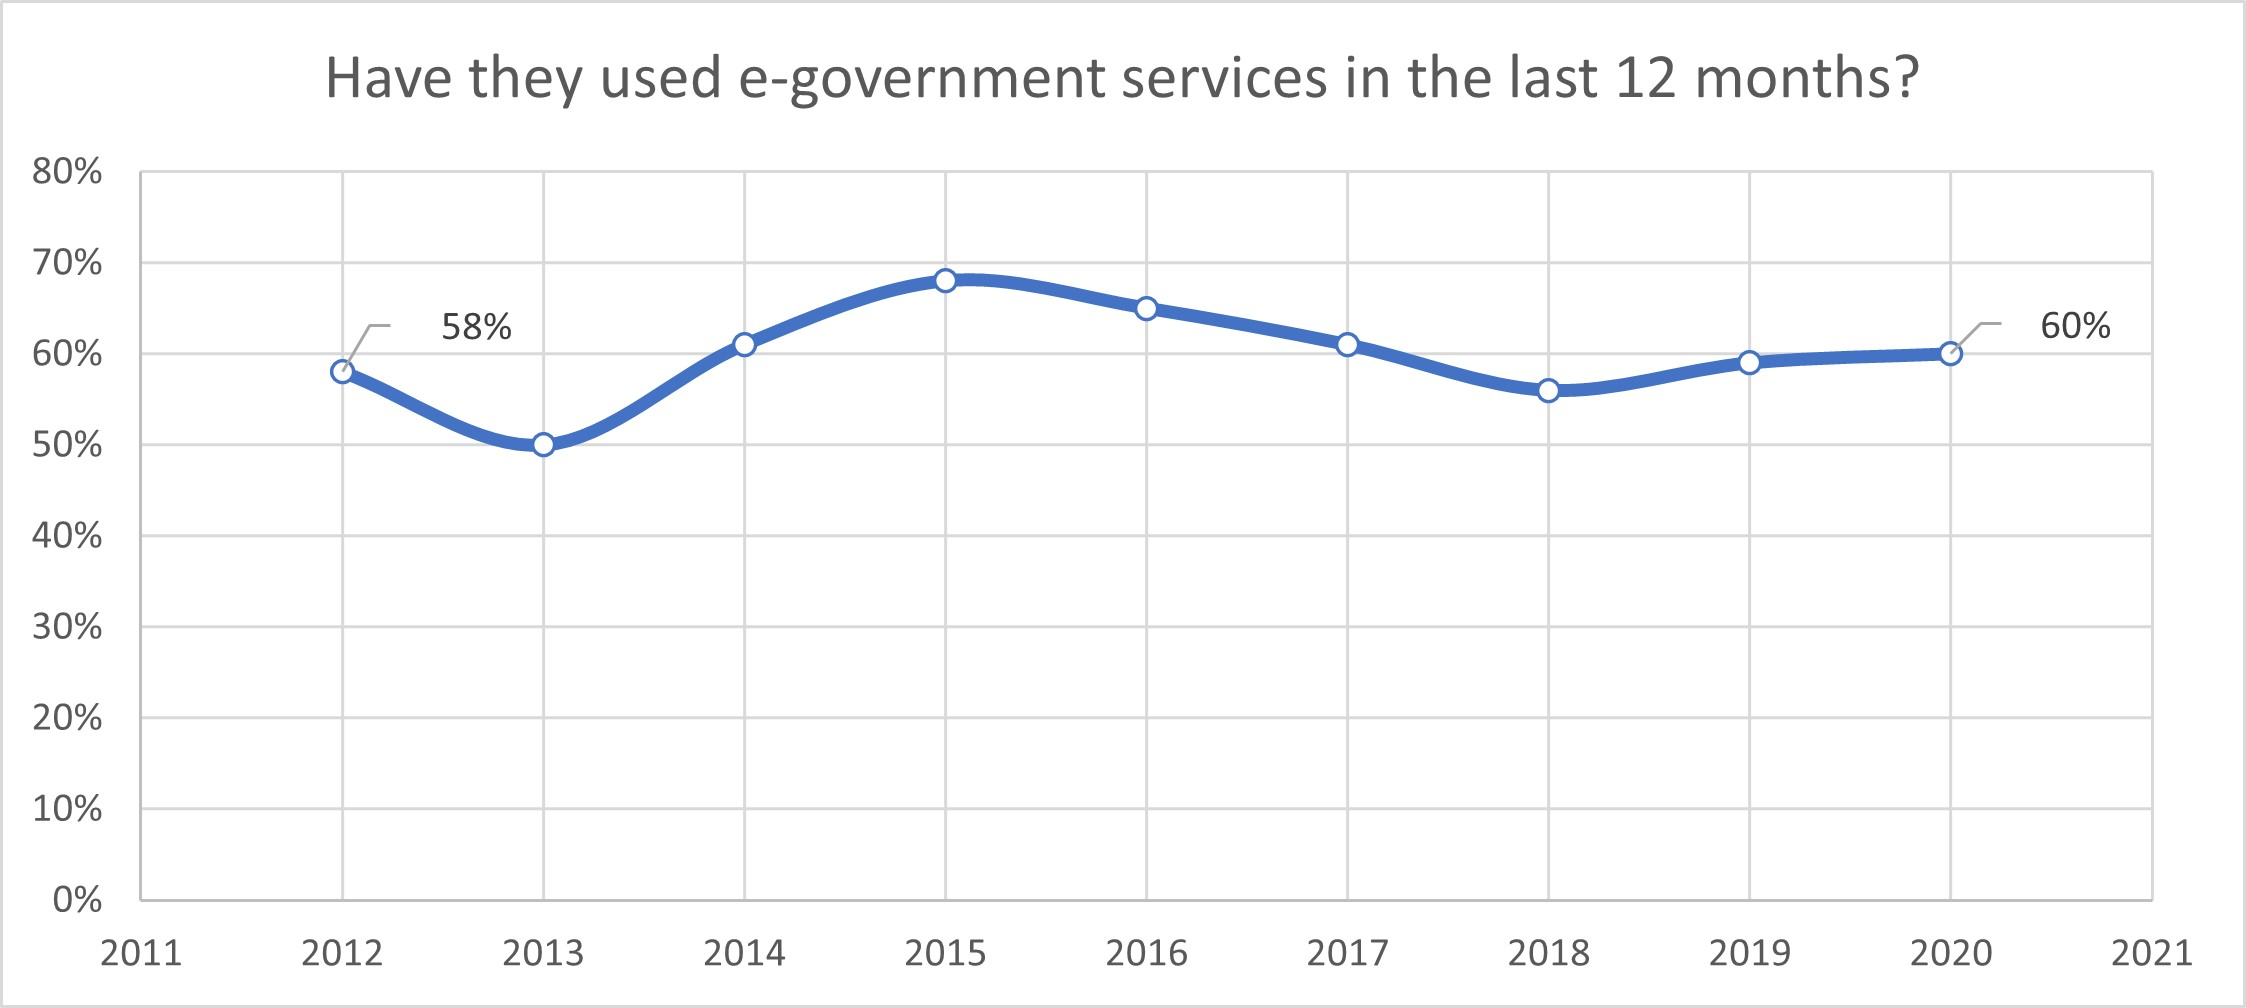
\includegraphics[width=1\textwidth]{images/tenYears.jpg}
\caption{Survey eGov in CH \cite{10years}}
\label{10years}
\end{figure}
\FloatBarrier

To understand how a country is positioned in this ranking, a benchmark is created every year, which monitors the development of eGovernment in Europe, based on specific indicators.\\
These indicators are divided by:
\begin{itemize}
\item User Centricity - indicates to what extent (information about) a service is
provided online and how this is perceived.
\item Transparency - indicates the transparency of the government for its responsibility, services and data in use.
\item Cross-Border Mobility - indicates to what extent EU citizens and businesses can use online services in another country.
\item Key Enablers - indicates the extent to which five technical pre-conditions are available online. These are eDocuments, eID, and Digital Post.
\end{itemize}

\newpage
Figure 3 describes the permformance of eGovernment in Switzerland in 2012 based on the indicators just described.
\begin{figure}[!htb]
\centering
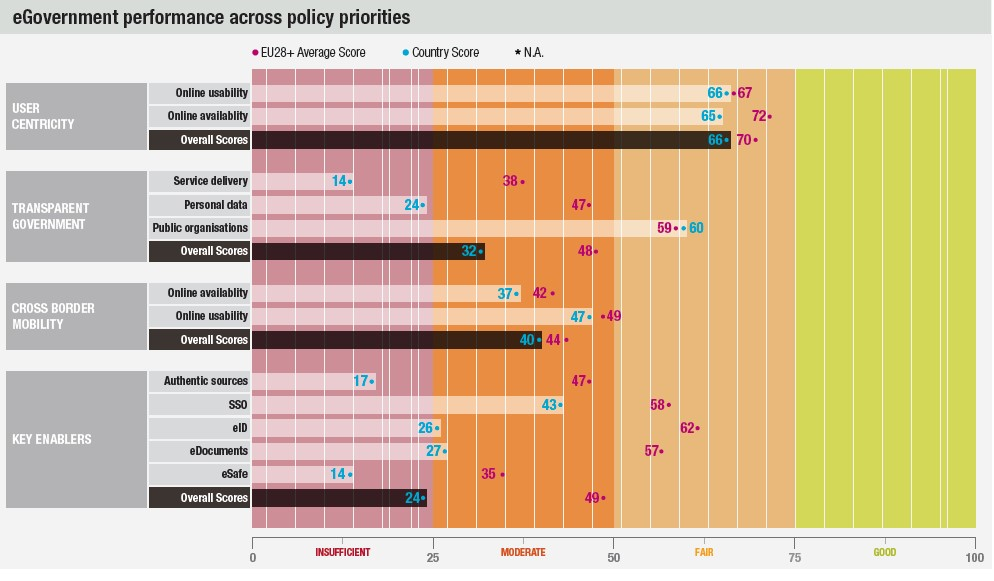
\includegraphics[width=1\textwidth]{images/key2012.jpg}
\caption{eGovernment Performance 2012 \cite{eGov2012bench}}
\label{bench2012}
\end{figure}
\FloatBarrier
https://joinup.ec.europa.eu/sites/default/files/inline-files/eGovernment%20in%20Switzerland%20-%20February%202016%20-%20Edition%2010_0%20-%20v3_00.pdf

What can be seen from Figure 3, is that Switzerland compared to the European average of 28 countries, on many indicators it is far behind.
With the results in hand, it was therefore decided to change the strategy so that the situation could be improved for the coming years.
This is why the eGovernment.ch team comes into play, which is fundamental for the improvement of the situation.

\subsubsection{eGovernment.ch Who's Who}

\textbf{Actual egovernment.ch actors}\\
The committee for the organization "e-government Switzerland" is as we said responsible for the strategies for everything related to the digitization of government in Switzerland and everything the federal government can offer the citizen.\\ 
Everything is available thanks to the site \url{https://www.egovernment.ch/}

%\begin{figure}[!htb]
%\centering
%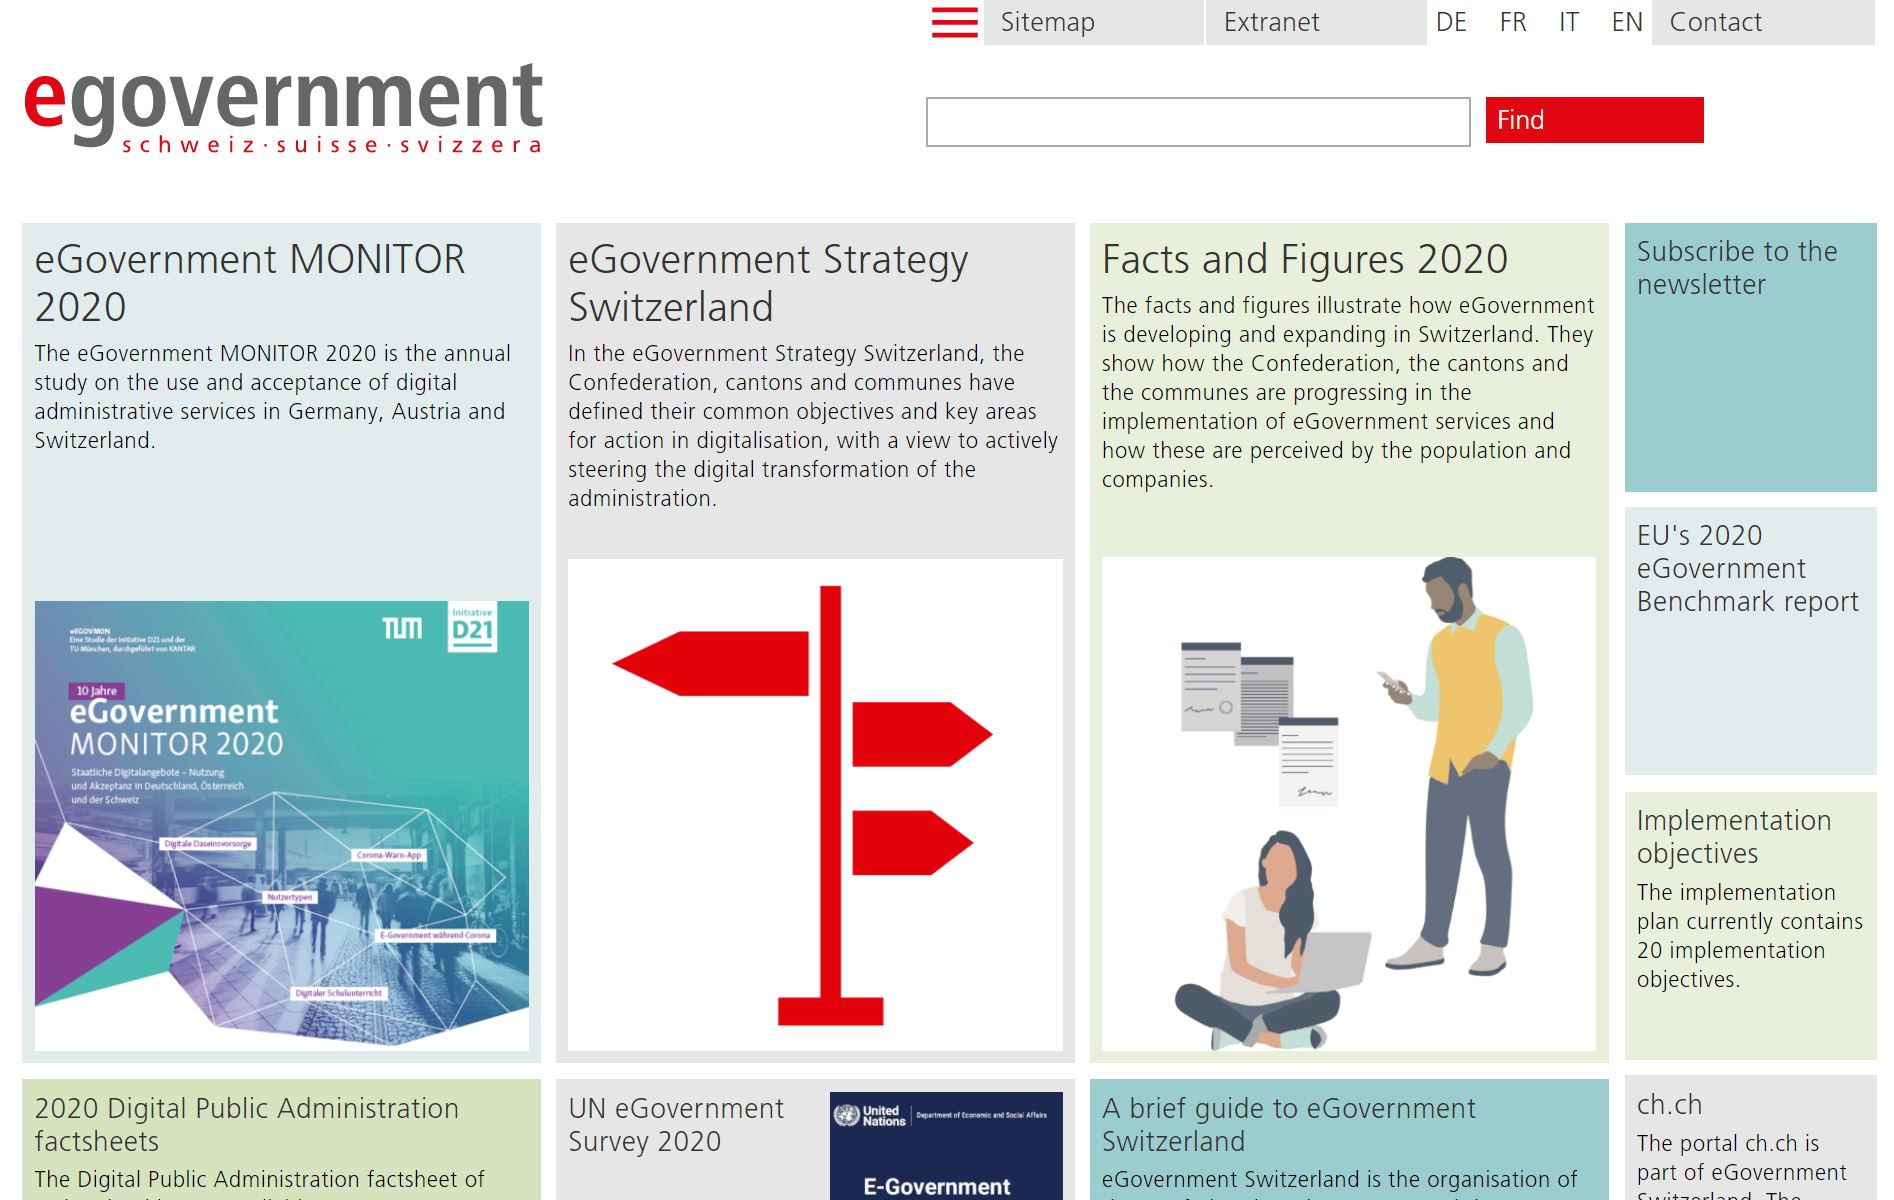
\includegraphics[width=1\textwidth]{images/egov.jpg}
%\caption{egovenment.ch Website \label{overflow}}
%\end{figure}
%\FloatBarrier

\begin{longtable}[ c ]{| m{3.5cm} | m{10cm}|}
\hline
\multicolumn{2}{| c |}{\textbf{eGovernment Members}}                                                                                                                                                      \\ \hline
\textbf{Name} & \textbf{Title and Function                                                                                               } \\ \hline
\endfirsthead
%
\multicolumn{2}{c}%
{{\bfseries Table \thetable\ continued from previous page}} \\
\hline
\textbf{Name} & \textbf{Title and Function                                                                                                  } \\ \hline
\endhead
%
Ueli Maurer & Federal Councillor, \acrfull{fdf}, chairman \\ \hline
Walter Thurnherr & Federal Chancellor,\acrfull{fch})\\ \hline
Marie-Gabrielle Ineichen-Fleisch & \acrfull{seco}\\ \hline
Maya Büchi-Kaiser & Cantonal Councillor of canton of Obwalden \\ \hline
Jean-Pierre Siggen & Cantonal Councillor of canton of Fribourg\\ \hline
Daniel Spadin  & Cantonal Chancellor  of canton of Grisons\\ \hline
Michael Künzle & Mayor of the city of Winterthur, canton of Zurich \\ \hline
Beat Tinner & Mayor of the commune of Wartau, canton of St. Gallen\\ \hline
Peter Bernasconi & representative of the Association of Swiss Communes\\ \hline
\caption{eGovernment Members}
\label{tab:eGovernment Members}\\
\end{longtable}

\subsubsection{Previous eGovernment Strategies}
In 2007, the Federal Council adopted the first national eGovernment strategy. With this strategy Switzerland tries to give a first touch to the general picture of eGovernment. Up to the end of 2015, this strategy was the basis for eGovernment cooperation between the Confederation, the cantons and the communes.\\

The table "eGovernment strategies 2008-2015" lists the objectives that the federal government has set itself for the years 2008-2015.\\


\begin{longtable}[ c ]{| m{4.5cm} | m{9cm}|}
\hline
\multicolumn{2}{|c|}{\textbf{eGovernment Strategies 2008-2015}} \\ \hline
\textbf{\begin{tabular}[c]{@{}l@{}}Organization responsible \\ for the implementation\end{tabular}} &
  \textbf{Description} \\ \hline
\endfirsthead
%
\multicolumn{2}{c}%
{{\bfseries Table \thetable\ continued from previous page}} \\
\hline
\textbf{\begin{tabular}[c]{@{}l@{}}Organization responsible \\ for the implementation\end{tabular}} &
  \textbf{Description} \\ \hline
\endhead
%
\acrshort{fitsu} &
  E-Government Architecture in Switzerland \\ \hline
EGovernment Switzerland &
  \begin{tabular}[c]{@{}l@{}}eCH platform for cantons and municipalities: \\ process exchange\end{tabular} \\ \hline
\acrshort{fitsu} &
  National eGovernment Map in Switzerland \\ \hline
\acrshort{sik}&
  \begin{tabular}[c]{@{}l@{}}eOperations Switzerland. Organization and \\ financing of eGovernment solutions used in common\end{tabular} \\ \hline
\acrshort{fitsu} &
  \begin{tabular}[c]{@{}l@{}}E-Government knowledge \\ management in the legal field\end{tabular} \\ \hline
\acrshort{swissdec} &
  \begin{tabular}[c]{@{}l@{}}Transmission of wage data from the accounting of \\ companies to the authorities and insurance companies\end{tabular} \\ \hline
simap.ch &
  Processing of public notices of competition \\ \hline
\acrshort{dcpa} &
  Building permit applications \\ \hline
\acrshort{foj} &
  \begin{tabular}[c]{@{}l@{}}Ordering and receiving certified extracts from registers, \\ civil status certificates, copies of important acts and \\ administrative decisions\end{tabular} \\ \hline
\begin{tabular}[c]{@{}l@{}}\acrshort{vsed}\end{tabular} &
  Notification of changes of address, arrivals, departures \\ \hline
Federal Chancellery &
  Electronic Vote \\ \hline
e-geo.ch &
  Easy and nationwide networked access to basic geodata \\ \hline
\acrshort{egris} &
  Computerized funds information system \\ \hline
\acrshort{hpi} &
  Suisse ePolice \\ \hline
\acrshort{foph} &
  Consumer protection parameters portal \\ \hline
Federal Chancellery &
  Electronic consultation procedure \\ \hline
Federal Tax administration &
  Electronic \acrshort{vat} Report \\ \hline
\acrshort{seco} &
  Authorizations in the field of work \\ \hline
Swiss Federal Archives &
  Open Government Data \\ \hline
\acrshort{fitsu} &
  \begin{tabular}[c]{@{}l@{}}Implementation of the cloud computing strategy \\ of the Swiss authorities\end{tabular} \\ \hline
\acrshort{fedpol} &
  \begin{tabular}[c]{@{}l@{}}Electronic identity recognized at national level \\ and in the European area\end{tabular} \\ \hline
\caption{eGovernment Strategies 2008-2015 \cite{resoconto2015}}
\label{tab:eGovernment Strategies 2008-2015}\\
\end{longtable}

\newpage
The table "Achievement of eGovernment strategies 2008-2015" lists the successes and milestones of this strategy.
 
\begin{longtable}[c]{| m{2.5cm} | m{11cm}|}
 \hline
 \multicolumn{2}{| c |}{\textbf{Achievement of eGovernment strategies 2008-2015}}\\
 \hline
 \textbf{Date} & \textbf{Description}\\
 \hline
 \endfirsthead
%
 \multicolumn{2}{c}%
 {{\bfseries Table \thetable\ continued from previous page}} \\
 \hline
 \textbf{Date} & \textbf{Description}\\
 \hline
 \endhead
%
 
 03.11.2009 & Consolidation of the organization for the eGovernment implementation project\\ \hline
 03.11.2009 & Forwarding of data to statistical offices\\ \hline
 04.11.2010 & Business between the compensation offices and their affiliates\\ \hline
 20.06.2011 & Standardization of personal data\\ \hline
 20.06.2011 & Swiss-wide standard for the exchange of electronic files and documents\\ \hline
 20.06.2011 & Electronic forms service\\ \hline
 20.06.2011 & SuisseID\\ \hline
 20.06.2011 & Founding of companies, communication of the changes\\ \hline
 20.06.2011 & Agricultural sector management\\ \hline
 24.10.2011 & Access to legal data\\ \hline
 24.10.2011 & Uniform inventory and reference database of public services\\ \hline
 24.10.2011 & Access to public electronic services (portals)\\ \hline
 24.10.2011 & Directory and competence service of the Swiss authorities\\ \hline
 05.04.2012 & Customs clearance of goods (import, export, transit)\\ \hline
 24.10.2012 & Legal basis for eGovernment\\ \hline
 24.10.2012 & Shared network infrastructure for all administrative levels\\ \hline
 10.06.2013 & Access to data from the Swiss Environment Observation Network\\ \hline
 10.06.2013 & Search and announcement of lost and found\\ \hline
 10.06.2013 & Electronic Archiving Service\\ \hline
 26.06.2014 & Data sharing regarding the reduction of insurance premiums\\ \hline
 20.02.2015 & Certifications of changes of civil status\\ \hline
 11.12.2015 & Services for the use of reference data in public administrations\\ \hline
\caption{Achievement of eGovernment strategies 2008-2015 \cite{resoconto2015}}
\label{tab:Achievement of eGovernment strategies 2008-2015}\\
\end{longtable}
Unfortunately as we have seen all these improvements were not enough, in fact in 2015 Switzerland was still at the bottom of the list of countries in Europe.
In 2015, the Steering Committee proposed a concrete new strategic direction so that the current strategy can be improved with a better performance.
Not only has it been decided to focus on a limited number of projects and tasks. To do this, the planning committee has increased the collaboration between the state levels.
A soft start for a Switzerland that faces the digital world.

\subsubsection{Just completed eGovernment Strategies}
The old strategy was in 2015 rivisited and replaced by the eGovernment Strategy Switzerland (2016-2019). The new strategy entered into effect immediately and developed in dialogue with representatives from business, science, research, and civil society. The key focus of the Strategy is on the development of a basic infrastructure to accelerate the development of eGovernment in Switzerland.\\

In the list are described the objectives that the federal government has set itself for the years 2016-2019:

\begin{longtable}[ c ]{| m{4.5cm} | m{9cm}|}
 \hline
 \multicolumn{2}{| c |}{\textbf{eGovernment Strategies 2016-2019}}\\
 \hline
 \textbf{\begin{tabular}[c]{@{}l@{}}Organization responsible \\ for the implementation\end{tabular}} &
  \textbf{Description} \\ \hline
\endfirsthead
%

 \multicolumn{2}{c}%
 {{\bfseries Table \thetable\ continued from previous page}} \\
 \hline
 \textbf{\begin{tabular}[c]{@{}l@{}}Organization responsible \\ for the implementation\end{tabular}} &
  \textbf{Description} \\
 \hline
 \endhead
%
 eOperations Switzerland AG & make the electronic notification service for change of address available throughout Switzerland\\ \hline
 Cantons Grisons, Schwyz and Zug  & online portal for the publication of election and voting results\\ \hline
 Federal Chancellery & extend the electronic voting offer to two thirds of the cantons\\ \hline
 FCh & improve access to online information of the authorities\\ \hline
 BFH, Swiss Federal Roads Office & Digital Vehicle Licence\\ \hline
 City of Bern & Ki-Tax: portal to submit online requests for complementary childcare to the family\\ \hline
 City of St. Gallen  & Chatbot for public administration\\ \hline
 Municipality of Moosseedorf (BE)  & Module allows municipalities to dialogue with citizens and discuss proposals with them.\\ \hline
 University of Applied Sciences of St. Gallen & Use of digital voice assistants for eGovernment services\\ \hline
 Canton of Fribourg & Progressive web applications for the population\\ \hline
 Canton of Geneva & Electronic identity and signature based on blockchain technologies\\ \hline
 CCGEO &  Up-to-date geodata that can be used extensively, durably, quickly and easily and in the quality required\\ \hline
 SECO & Allow companies to process the practices of the Confederation and the cantons electronically in a single place\\ \hline
 ESTV SuisseTax & To make the VAT report without discontinuity of the transmission systems \\ \hline
 Swissdec & Simplify the electronic exchange of financial data between companies and insurers and the authorities that are members of Swissdec\\ \hline
 Eidgenössische Finanzverwaltung (EFV) & Promote the use of e-invoices to the Confederation, cantons and municipalities\\ \hline
 Schweizerisches Bundesarchiv (BAR) & Implementation of the Open Government Data Strategy Switzerland 2014-2018\\ \hline
 SECO & Simplify the registration procedure for eGovernment platforms with a prototype of the Swiss Federation of Identity (SFI).\\ \hline
 FOJ for legislation, Fedpol for the concept and implementation & Create a state-recognized electronic identity that allows the Swiss population to handle administrative tasks online.\\ \hline
 Federal IT control body (FSUIT), eOperations Switzerland & Easy verification of the authenticity and integrity of a document with digital signature\\ \hline
 SIK & Development of eOperations Switzerland\\ \hline
 FOJ & Establish a common address service for the authorities\\ \hline
 FOJ & Property search with the AHV number\\ \hline
 Association eCH & Promote the development and use of e-government standards\\ \hline
 SIK & Making it possible to carry out pilot projects and studies to consolidate eGovernment\\ \hline
 eJustice.CH association & Promote the exchange of knowledge and experience on legal issues concerning eGovernment\\ \hline
 Federal Archives & Modeling and implementation of a data inventory\\ \hline
 Canton of Jura and Fribourg & The two cantons founded the igovportal.ch association, which is responsible for managing and developing the iGovPortal virtual counter solution.\\ \hline
 Canton of Fribourg & The canton has developed a signature system that allows you to log in with the digital identities of different providers to perform an online service and to sign in electronically.\\ \hline
 AHV/IV & Introducing digitization in the first pillar sector through automated specialist processes and electronic data exchange\\ \hline
 Federal Office for Statistics (BFS) & Professional and technical harmonization and standardization of the exchange of register data\\ \hline
 Association eGov-Switzerland, Association eCH & Provide support to authorities in the development of process management and inter-federal collaboration\\ \hline
 \caption{eGovernment Strategies 2016-2019 \cite{eGov2016Strat}}
 \label{tab:eGovernment Strategies 2016-2019}\\
\end{longtable}
So many projects are on the list but the focal points of the 2016-2019 strategy of "eGovernment.ch" are eMovingCH, EasyGov, eOperations,\acrshort{evote}, \acrshort{eid}.

\paragraph{eMovingCH} is the solution for electronic move notification eMovingCH is now reachable for more than half the population.
\paragraph{EasyGov} is the online portal for companies to centralize, facilitate and optimize the administrative procedures that are mandatory for Swiss companies.
\paragraph{\acrshort{evote}} is the possibility to vote online. The cantons are gradually introducing this service at the moment are less than half because still in the experimental phase.
%\url{https://www.swissinfo.ch/eng/expat-voting_swiss-e-voting-system-to-undergo--hacker-test-/44539598}
%adesso evoting (vari progetti fra cui bfh)
\paragraph{\acrshort{eid}}
on March 20, 2018 the national council introduced the digital identity (\acrshort{eid}). The population will be able to use online services provided by authorities and companies.
The federal government is responsible for the identification of persons.

The table "Achievement of eGovernment strategies 2016-2019" lists the successes and milestones of this strategy in detail.

\begin{longtable}[ c ]{| m{0.8cm} | m{13.5cm}|}
 \hline
 \multicolumn{2}{| c |}{\textbf{Achievement of eGovernment strategies 2016-2019}}\\
 \hline
 \textbf{Date} & \textbf{Description}\\
 \hline
 \endfirsthead
%
 \multicolumn{2}{c}%
 {{\bfseries Table \thetable\ continued from previous page}} \\
 \hline
 \textbf{Date} & \textbf{Description}\\
 \hline
 \endhead
%
  
 2016 & The Canton of Zurich is the first canton to have introduced eMovingCH. In August, the City of St. Gallen did the same and at the end of 2016 the solution was adopted by most of the municipalities in the Canton of Zurich. \\ \hline 
2016 & Common infrastructure for cantonal e-government portals.
 The Canton of Jura, in cooperation with the Canton of Fribourg, has created the conditions for several authorities to share the same infrastructure, i.e. a portal for eGovernment. Since 2019 this solution has been used by the cantons of Jura, Freiburg, Solothurn and St. Gallen. \\ \hline
Jan 2017 &  Since the beginning of 2017, the section www.egovernment.ch/recht (in German and French) presents comprehensive documentation on legal issues related to eGovernment.\\ \hline
Jan 2017 & Since January the electronic signature validation system is also used by the authorities of the Canton of Zug. Individuals and businesses can thus verify the authenticity and integrity of PDF documents digitally signed by the Canton of Zug.\\ \hline
Oct 2017 & Federal Councillor Ueli Maurer signed the European Declaration on eGovernment ("Tallinn Declaration on eGovernment"). Switzerland is committed to the implementation of six principles, including data retention, transparency and interoperability in the digitization of the administration.\\ \hline
Nov 2017 & With the launch of the EasyGov portal, \acrfull{seco} has realized a key point on the portal dedicated to companies. The portal enables companies to process online their files with federal, cantonal and municipal authorities using a single platform.\\ \hline
Apr 2018 & Since the beginning of April, the value added tax report can be submitted in \acrshort{xml} format on the portal of the Federal Tax Administration SuisseTax. This makes it possible to report \acrshort{vat} electronically without interruptions in the transmission systems.\\ \hline
Jun 2018 & eOperations Switzerland is born. eOperations Switzerland was one of the priorities expressed upstream of the development of the eGovernment Strategy Switzerland 2016-2019.\\ \hline
Oct 2018 & Thanks to new electronic participatory solutions, citizens can interact in an innovative way in social and political processes. The municipalities of Moosseedorf (BE), Sargans (SG) and Untereggen (SG) have developed, in collaboration with the Association of Swiss Municipalities (ACS) and the ch.ch platform, a participation module that makes dialogue between public authorities and citizens possible.\\ \hline
Jun 2019 & The Steering Committee of "eGovernment Switzerland" submitted the draft of the eGovernment Strategy 2020-2023 for consultation to the Confederation, the cantons and the municipalities. Based on the "digital first" principle, the strategy aims to make the electronic channel the first choice for administrative processes. \\ \hline
Sep 2019 & On the occasion of Digital Day 2019, the organization "e-government Switzerland", together with several partner organizations, explained how easy it is to do administrative work online. \\ \hline
Sep 2019 &  On September 27, the Parliament approved the \acrshort{eid} law. Thanks to a state-recognized electronic identity, the Swiss population will be able to use the online services provided by the authorities and companies, thus avoiding the need to re-register each time.\\ \hline
Oct 2019 & The eMovingCH solution was adopted by 13 cantons (as of October 2019). This means that more than half of the inhabitants of Switzerland can fulfill their personal notification obligations in connection with the move directly on the eMovingCH portal.\\ \hline
 \caption{Achievement of eGovernment strategies 2016-2019 \cite{eGov2016Strat}}
 \label{tab:Achievement of eGovernment strategies 2016-2019}\\
\end{longtable}

This strategy has increased collaboration between the three levels of government and shown that this collaboration is paying back.
This collaboration has also made it possible for cantons, municipalities and the confederation to expand eGov on the territory, so that there are some cantons where eGov is already working, others where it is planned and only a couple where it hasn't started yet.
In figure 4 it is possible to see a map of the extension of the eGov on the territory.
\begin{figure}[ht!]
\centering
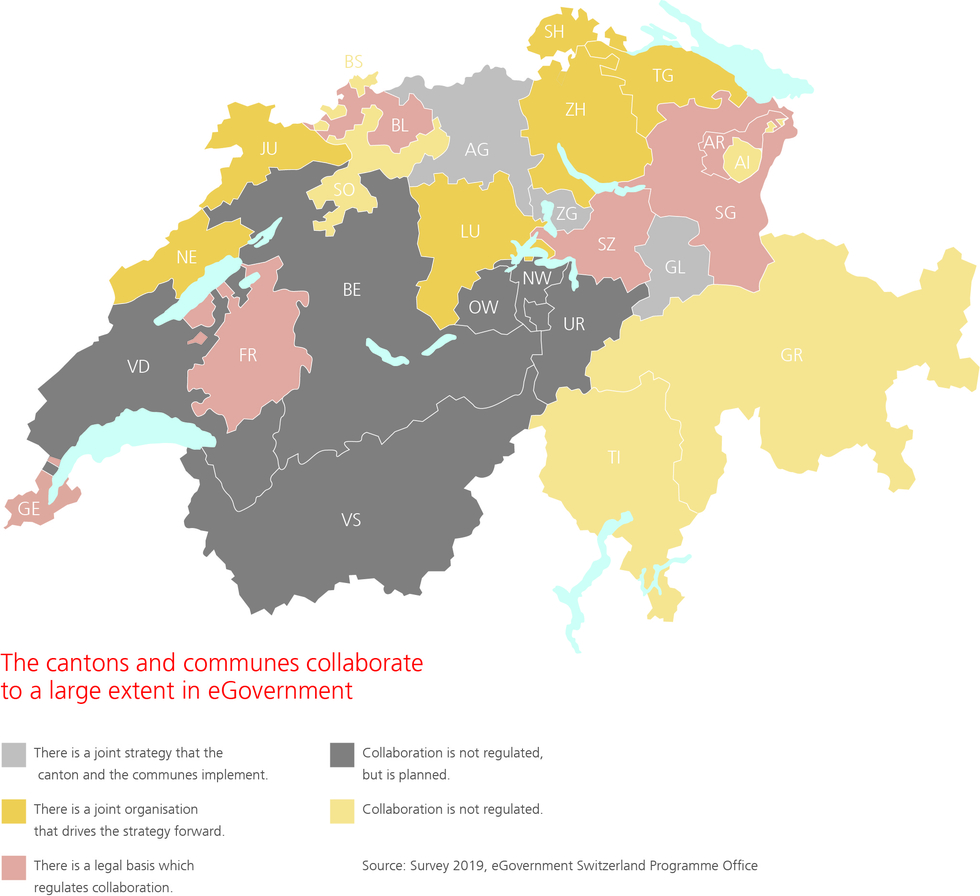
\includegraphics[width=1\textwidth]{images/survey2019.jpg}
\caption{Swiss expansion map e-gov 2019 \cite{fact2020}}
\label{egov2019}
\end{figure}
\FloatBarrier

These results have taken Swiss eGovernment to the next step: after the 2008-2015 strategy, eGovernment was still immature, but now we have much more to offer.

\newpage
\subsubsection*{Swiss in 2018}
At the end of this eGov strategy (2018) we can see a clear increase in Switzerland's indicators compared to the old ranking.
Not only that it also improved in comparison to many European countries.\\
In figure 5 we can see the Swiss perfomance in 2018:
\begin{figure}[!htb]
\centering
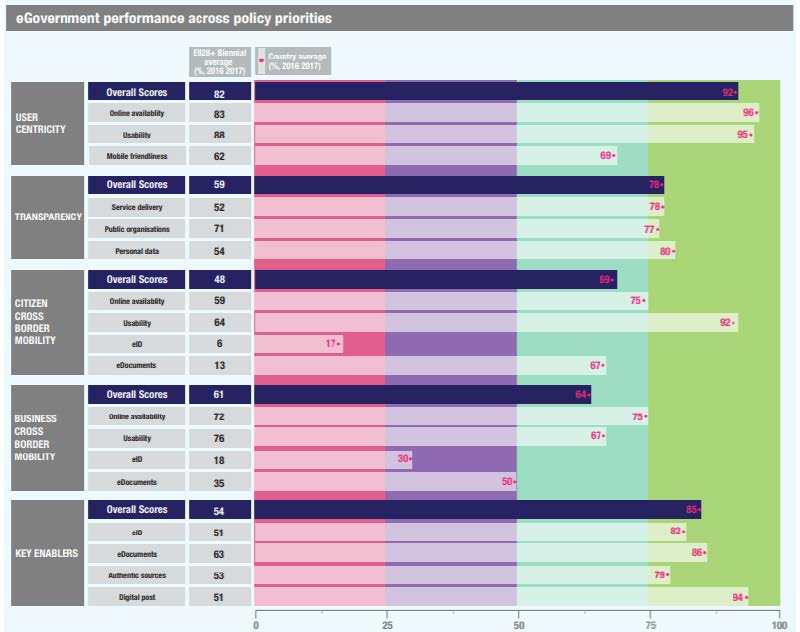
\includegraphics[width=1\textwidth]{images/key2018.jpg}
\caption{eGovernment Performance 2018 \cite{eGov2018bench}}
\label{bench2018}
\end{figure}
\FloatBarrier
%prospettiva attuale: 
%\url{https://www.egovernment.ch/it/dokumentation/controll/}\\
%foto da flickr: \url{https://www.flickr.com/photos/initiatived21/albums/72157716529142517/with/50504905707/}\\

\subsubsection*{Lesson learned?} 
At the end of 2019 and so at the conclusion of the strategy, the commitee can be more than satisfied.
The electronic channel is now the first choice for contacting authorities, although electronic services are not yet fully available, so many people still have to go in person or use letters.
The population in general is satisfied with eGov, in fact once a person has used an e-service for administrative tasks he often continues to use this e-service, preferring it to the traditional method. Nearly more than 70\% of the population prefers to fill out their tax forms online.

Thanks to EasyGove.swiss Swiss companies have been able to save almost 47 million CHF, almost 9000 users are registered on the portal.*

Although more than 47\% of the population prefers electronic voting, unfortunately it is not yet widely available, this point will be continued in the next strategy, as well as improving e-ID.

Source: eGovernment Monitor 2018 \cite{eGov2018Monitor}, \acrshort{seco}*

%\url{https://www.egovernment.ch/en/dokumentation/facts-and-figures/facts-and-figures-2019/}

%https://www.egovernment.ch/en/dokumentation/facts-and-figures/facts-and-figures-2017/

\subsubsection{eGovernment Present/Future Strategy}
The 2016-2019 strategy has come to an end, leaving many more goals for the future. The lesson from the first strategy to this one, which is the third, has been learned. In fact, the eGovernment.ch Committee comes back stronger than before wanting to modify, improve and expand the points that in the just concluded strategy were critical to the completeness of eGovernment.

In the table eGovernment Strategies 2020-2023 are listed the next steps that have emerged and not concluded from the previous strategy.\\

\begin{longtable}[c]{| m{2cm} | m{11.5cm}|}

 
 \hline
 \multicolumn{2}{| c |}{\textbf{eGovernment Strategies 2020-2023}}\\
 \hline
 \textbf{Topic} & \textbf{Implementation objective}\\
 \hline
 \endfirsthead
%
 \multicolumn{2}{c}%
 {{\bfseries Table \thetable\ continued from previous page}} \\
 \hline
 \textbf{Topic} & \textbf{Implementation objective}\\
 \hline
 \endhead
%
 
 \multirow{4}{*}{eService} 
 & • Expand EasyGov.swiss\\  
 & • Extend eMovingCH to the whole of Switzerland\\ 
 & • Reorient eVoting and ensure stable trial operation \\
 & • Establish signature validator throughout Switzerland\\
 \hline
 Participation & • Promoting eParticipation projects at communal and cantonal levels\\
 \hline
 \multirow{2}{*}{Access} 
 & • Establish cross-authority eInformation and operation of the new ch.ch website\\
 & • Improve user-friendliness of eGovernment services\\
 \hline
 IAM & • Implement \acrshort{eid}\\
 \hline
 \multirow{3}{*}{Data} 
 & • Establish a cross-authority master data management system\\
 & • Establish a national address service\\
 & • Make anonymous and non-confidential data from the Confederation, cantons and communes freely accessible\\
 \hline
 Standards & • Promote standardisation\\
 \hline
 \multirow{2}{*}{Architecture} 
 & • Develop and manage eGovernment architecture for the strategic implementation plan\\
 & • Develop a concept for the traceability of the use of personal data\\
 \hline
 \multirow{3}{*}{Organisation} 
 & • Support innovative projects\\
 & • Promote the administration's data platforms\\
 & • Support public projects in the areas of information technology and eGovernment\\
 \hline
 Legal & • Offer advice and coordination in legal matters\\
 \hline
 Trust & • Strengthen the public and businesses' trust in eGovernment services\\
 \hline 
 Knowledge & • Promote knowledge of the potential benefits of digital processes in public administration\\ 
 \hline
 \caption{eGovernment Strategies 2020-2023 \cite{eGov2020Strat}}
 \label{tab:eGovernment Strategies 2020-2023}\\
\end{longtable}

\subsection{Present situation}
The current strategy includes many innovative projects using new technologies and more cooperation among all three federal levels. 
In the last 5 years, Switzerland has become more digital, with 93\% of households using the Internet, an improvement of 10\%\cite{fact2020}.
In the 15-55 age group, internet usage is as high as 100\%.
This increase in daily internet usage has caused many users to become more skilled in the use of digital technologies and tools.
In fact, nearly 70\% of the population in the past year has searched for information on administrative e-portals, 60\% has downloaded forms, and about half has filled out forms online.

A survey shows that the majority of the Swiss population does not use online services because they are not informed about them or because they are afraid of the security of their personal data; this is an auspicious sign for the future. The population is also asking the authorities for more transparency in the procedures and use of personal data.\\
Source: eGovernment Monitor 2019\cite{eGov2019Monitor}\\

All of these improvements have moved Switzerland up in the European picture, Figure 6 shows that Switzerland's Achilles heel is \acrlong{eid} and transparency, while all other factors are in the average or above.\\
\newpage
Swiss perfomance in 2020
\begin{figure}[!htb]
\centering
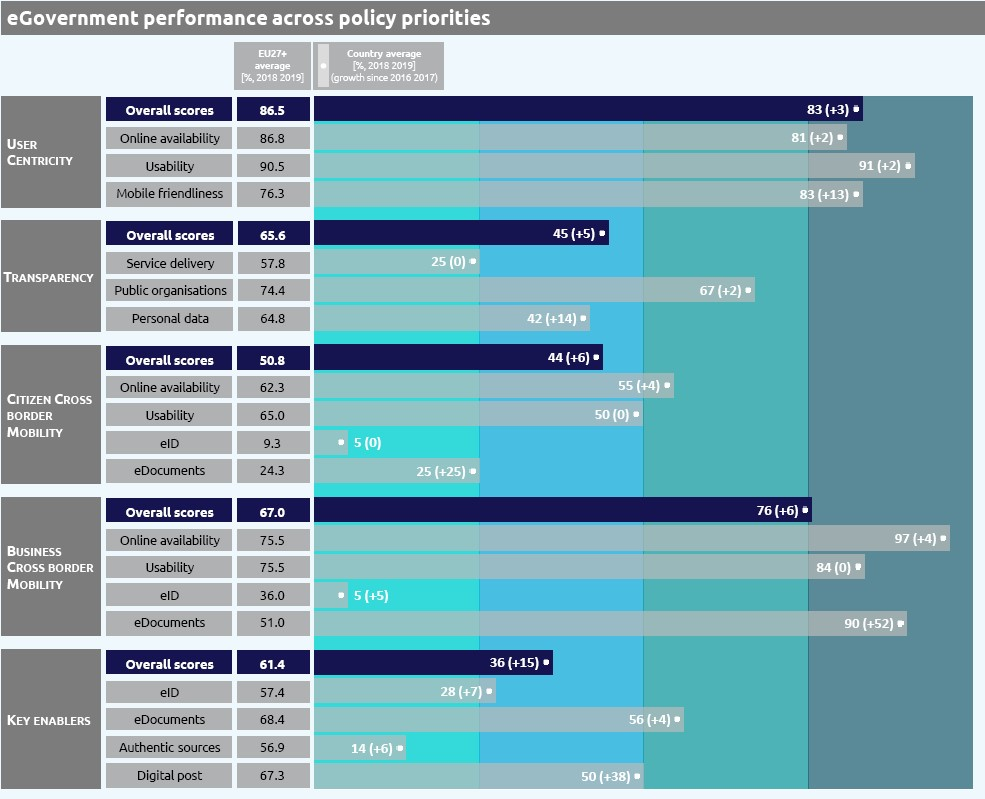
\includegraphics[width=1\textwidth]{images/key2020.jpg}
\caption{eGovernment Performance 2020 \cite{eGov2020bench}}
\label{egov2020}
\end{figure}
\FloatBarrier

\subsubsection*{Comparison}
When the topic is electronic government, the nation that needs to be mentioned is Estonia.
I take this country as an example because it is the most advanced in the world in terms of electronic government, in fact 99\% of the population has an e-ID of which 70\% use it regularly, in addition to the fact that 99\% of government services are online.
However, it must be said that Estonia started in 1994 the implementation of its government much earlier than Switzerland.
Not to forget the size, Estonia's population is only 1.3 million compared to Switzerland's 8.6 million.
The smaller the country the easier the management, for this reason it is difficult to make a comparison, rather you can use Estonia's e-government as an example.

Source: Estonia website \cite{Estonia}

\subsection{Covid}
Around the end of 2019, the world was hit by a pandemic, which turned our ways upside down.
\subsubsection*{What has changed with covid?}
Rules for social distancing and working from home were introduced at the end of March, the government urged the population to stay at home as much as possible, schools meanwhile closed their on-site classes, effectively moving the population online.

\subsubsection*{Government and covid}
The government through the BAG has used its telematic channels to inform the population, then with press conferences on live TV, on all portals belonging to the confederation (admin and ch).
In order to track the disease, the SwissCovid app has been released although the effectiveness is unknown since it is used well by few.

Thanks to the coordination of Daniel Koch, "Mr Coronavirus", head of the BAG during the first pandemic wave, the government has spent more than 15 million francs in information for covid, but after his retirement the government has lost its figurehead, de facto going into chaos.

BAG can be reached through: \href{https://www.bag.admin.ch/bag/en/home.html}{\emph{www.bag.admin.ch}}

\subsubsection*{Pandemic and vote}
The disease raises the issue of digital democracy, because of covid the work of the government, and not only, has slowed down a lot and in some cases had to stop; meetings canceled or postponed, signatures suspended and other inconveniences.
However, thanks to the situation it was a test for democracy, in fact to avoid cancelling other appointments we had to adapt by introducing an electronic voting system, at least for parliamentarians.
It is not an isolated case only in Switzerland, other parliamentarians around the world have had to test similar tools in this period, demonstrating that the digital way is possible and safer in cases of emergency, although always with the problem of secrecy of the vote and avoid any risk of falsification of it.
The crisis will certainly encourage the development of these digital tools, certainly pushing much more on electronic voting.
Not only that, it has certainly opened the eyes of technology skeptics, making them realize that in this case it is more than necessary for the survival of the government and its institutions.\\

In the months between June and December there were several online votes throughout Switzerland and in November the first election of a chairman of a party in Canton Ticino, a ballot that lasted several hours due to technical difficulties.

\subsubsection*{What people think and how they use eGov}
A survey was done during the coronavirus crisis, and in Switzerland, 12\% of respondents said they had processed administrative paperwork electronically more often during the pandemic. During this period, 3\% used an online service for the first time. The main reason, circa 30\%, was to avoid going to an office in person. Approximately 60\% of users who handled administrative paperwork electronically during the COVID-19 crisis said they were satisfied with the service and the response time of the authorities. The crisis has changed people's mindset about online services. 70\% of all interviewees intend to use online services more frequently even after the pandemic crisis.\cite{eGov2020Monitor}

\newpage

\subsection{eGovernment Services for Citizens}
The European Commission and the Member States thanks to \href{https://europa.eu/youreurope/citizens/index_en.htm}{\emph{Your Europe initiative}} have drawn up a series of basic public services for the population, and is categorized as follows:
\begin{enumerate}
\setlength{\itemsep}{0pt}
\setlength{\parskip}{0pt}
\item Travel
\item Work and retirement
\item Vehicles
\item Residence formalities
\item Education and youth
\item Health and Family
\item Consumers.
\end{enumerate}

\begin{table}[h!]
\renewcommand\arraystretch{1.2}
\begin{tabular}{ | m{4cm} | m{9cm} | }
\hline
\multicolumn{2}{ | c | }{List of all the websites:} \\
\hline
\multirow{3}{*}{Travel} & \url{http://www.schweizerpass.admin.ch}\\
& \url{https://www.ch.ch/en/passport-id-card/}\\
& \url{https://www.sem.admin.ch/sem/de/home.html}\\ \hline

\multirow{4}{*}{Work and Money} & \url{https://www.arbeit.swiss/}\\ 
 & \url{https://www.ch.ch/en/employment/}\\
 & \url{https://www.ch.ch/en/reference/}\\
 & \url{https://www.belogin.directories.be.ch/}\\ \hline
 
\multirow{2}{*}{Vehicles} & \url{https://www.uvek.admin.ch/}\\
 & \url{https://www.ch.ch/en/driving-licence/}\\ \hline
 
\multirow{3}{*}{Residence formalities} & \url{https://www.eumzug.swiss/}\\
 & \url{https://www.fedpol.admin.ch/}\\
 & \url{https://www.swissid.ch/}\\ \hline
 
\multirow{3}{*}{Education} & \url{https://www.sbfi.admin.ch/}\\
 & \url{https://www.swissuniversities.ch/}\\
 & \url{https://www.nb.admin.ch/}\\ \hline
 
\multirow{4}{*}{Health and Family} & \url{https://www.ch.ch/en/insurance-social-security/}\\
 & \url{https://www.ch.ch/en/marriage/}\\
 & \url{https://www.ch.ch/en/divorce/}\\
 & \url{https://www.ch.ch/en/registered-partnership/}\\ \hline
 
Consumers & \url{https://www.kmu.admin.ch/kmu/en/home/concrete-know-how/sme-management/e-commerce.html}\\ \hline

\end{tabular}
\caption{List of all the websites}
\end{table}

\newpage

\subsubsection{Travel}
\begin{center}
\begin{tabular}{m{2.5cm} m{12cm}} 
\hline
\multicolumn{2}{ | l | }{\textbf{Passport}} \\
\hline
Responsibility: & 'Passeport Suisse', Federal Office of Police, individual cantons and communes \\[1ex]
Website: & \href{http://www.schweizerpass.admin.ch}{\emph{http://www.schweizerpass.admin.ch}},\href{https://www.ch.ch/en/passport-id-card/}{\emph{https://www.ch.ch/en/passport-id-card/}}\\[1ex]
Description: & Switzerland issues biometric passports with electronic chips that contain all the necessary data. You can get all the information about them online, then you will have to contact the municipality or canton of residence for the application.
\end{tabular}
\end{center}

\begin{center}
\begin{tabular}{m{2.5cm} m{12cm}} 
\hline
\multicolumn{2}{ | l | }{\textbf{Permanent residence permit}} \\
\hline
Responsibility: & \acrfull{sem}, Cantons\\[1ex]
Website: & \href{https://www.sem.admin.ch/sem/de/home.html}{\emph{https://www.sem.admin.ch/sem/de/home.html}}\\[1ex]
Description: & Information about all the residence permits present, and how to apply to the cantons.
\end{tabular}
\end{center}

\subsubsection{Work and retirement}
\begin{center}
\begin{tabular}{m{2.5cm} m{12cm}}
\hline
\multicolumn{2}{ | l | }{\textbf{Job search services}} \\
\hline
Responsibility: & \acrshort{seco}\\[1ex]
Website: & \href{https://www.arbeit.swiss/}{\emph{https://www.arbeit.swiss/}}\\[1ex]
Description: & Online database that connects job seekers, job providers, federal and cantonal institutions.
\end{tabular}
\end{center}

\begin{center}
\begin{tabular}{m{2.5cm} m{12cm}} 
Responsibility: & Federal Chancellery, Cantons\\[1ex]
Website: & \href{https://www.ch.ch/en/employment/}{\emph{https://www.ch.ch/en/employment/}},\href{https://www.ch.ch/en/reference/}{\emph{https://www.ch.ch/en/reference/}}\\[1ex]
Description: & Detailed information at the service of the citizen who connects him/her to everything related to work.
\end{tabular}
\end{center}

\begin{center}
\begin{tabular}{m{2.5cm} m{12cm}}
\hline
\multicolumn{2}{ | l | }{\textbf{Tax}} \\
\hline 
Responsibility: & Severals cantons\\[1ex]
Website: & \href{https://www.belogin.directories.be.ch/}{\emph{https://www.be.ch/belogin/}}\\[1ex]
Description: & service to pay taxes in the canton Bern.
\end{tabular}
\end{center}

\subsubsection{Vehicles} 
\begin{center}
\begin{tabular}{m{2.5cm} m{12cm}}
\hline
\multicolumn{2}{ | l | }{\textbf{Transport and Communication}} \\
\hline 
Responsibility: & \acrfull{detec}\\[1ex]
Website: & \href{https://www.uvek.admin.ch/}{\emph{https://www.uvek.admin.ch/}}\\[1ex]
Description: & Detailed information about energy, transport , environment and comunication.
\end{tabular}
\end{center}

\begin{center}
\begin{tabular}{m{2.5cm} m{12cm}} 
\hline
\multicolumn{2}{ | l | }{\textbf{Driving licence}} \\
\hline 
Responsibility: & Cantons and communes\\[1ex]
Website: & \href{https://www.ch.ch/en/driving-licence/}{\emph{https://www.ch.ch/en/driving-licence/}}\\[1ex]
Description: & Detailed information about driving licence and in which canton it is appropriate to apply.
\end{tabular}
\end{center}

\subsubsection{Residence formalities}
\begin{center}
\begin{tabular}{m{2.5cm} m{12cm}} 
\hline
\multicolumn{2}{ | l | }{\textbf{Moving home}} \\
\hline 
Responsibility: & Confederation, Cantons and communes\\[1ex]
Website: & \href{https://www.eumzug.swiss/}{\emph{https://www.eumzug.swiss/}}, \href{https://www.ch.ch/en/moving/}{\emph{https://www.ch.ch/en/moving/}}\\[1ex]
Description: & Everything you need to know to move from one municipality to another, simplifying bureaucracy.
\end{tabular}
\end{center}
 
\begin{center}
\begin{tabular}{m{2.5cm} m{12cm}} 
\hline
\multicolumn{2}{ | l | }{\textbf{Police}} \\
\hline 
Responsibility: & \acrfull{fedpol}\\[1ex]
Website: & \href{https://www.fedpol.admin.ch/}{\emph{https://www.fedpol.admin.ch/}}\\[1ex]
Description: & \acrshort{fedpol} coordinates, analyses and investigates complex cases involving serious crime
\end{tabular}
\end{center}

\begin{center}
\begin{tabular}{m{2.5cm} m{12cm}}
\hline
\multicolumn{2}{ | l | }{\textbf{\acrshort{eid}}} \\
\hline  
Responsibility: & \acrshort{seco}, SwissSign Group\\[1ex]
Website: & \href{https://www.swissid.ch/}{\emph{https://www.swissid.ch/}}\\[1ex]
Description: & Free service provided by SwissSign Group, a joint venture of state-affiliated businesses, financial institutions, insurance and health insurance companies.
\end{tabular}
\end{center}

\subsubsection{Education and youth} 
\begin{center}
\begin{tabular}{m{2.5cm} m{12cm}}
\hline
\multicolumn{2}{ | l | }{\textbf{School}} \\
\hline  
Responsibility: & \acrfull{seri}\\[1ex]
Website: & \href{https://www.sbfi.admin.ch/}{\emph{https://www.sbfi.admin.ch/}}\\[1ex]
Description: & is a service that covers everything related to education, research and innovation.
\end{tabular}
\end{center}

\begin{center}
\begin{tabular}{m{2.5cm} m{12cm}} 
\hline
\multicolumn{2}{ | l | }{\textbf{University}} \\
\hline 
Responsibility: & Confederation, University Rectors Committee\\[1ex]
Website: & \href{https://www.swissuniversities.ch/}{\emph{https://www.swissuniversities.ch/}}\\[1ex]
Description: & The common voice of the Swiss universities and promotes cooperation and coordination between the universities and the various types of universities.
\end{tabular}
\end{center}

\begin{center}
\begin{tabular}{m{2.5cm} m{12cm}} 
\hline
\multicolumn{2}{ | l | }{\textbf{Swiss National Library}} \\
\hline 
Responsibility: & \acrfull{fdha}\\[1ex]
Website: & \href{https://www.nb.admin.ch/}{\emph{https://www.nb.admin.ch/}}\\[1ex]
Description: & collects, catalogues and stores information about Switzerland and makes it accessible to all.
\end{tabular}
\end{center}

\subsubsection{Health and Family}
\begin{center}
\begin{tabular}{m{2.5cm} m{12cm}} 
\hline
\multicolumn{2}{ | l | }{\textbf{Health insurance}} \\
\hline 
Responsibility: & Federal Chancellery, Cantons\\[1ex]
Website: & \href{https://www.ch.ch/en/insurance-social-security/}{\emph{https://www.ch.ch/en/insurance-social-security/}}\\[1ex]
Description: & Detailed information for everything related to mandatory insurances.
\end{tabular}
\end{center}

\begin{center}
\begin{tabular}{m{2.5cm} m{12cm}} 
\hline
\multicolumn{2}{ | l | }{\textbf{Marriage}} \\
\hline 
Responsibility: & Federal Chancellery, Municipalities\\[1ex]
Website: & \href{https://www.ch.ch/en/marriage/}{\emph{https://www.ch.ch/en/marriage/}}\\[1ex]
Description: & Detailed bureaucratic information for everything related to marriage.
\end{tabular}
\end{center}

\begin{center}
\begin{tabular}{m{2.5cm} m{12cm}} 
\hline
\multicolumn{2}{ | l | }{\textbf{Divorce}} \\
\hline 
Responsibility: & Federal Chancellery, Municipalities\\[1ex]
Website: & \href{https://www.ch.ch/en/divorce/}{\emph{https://www.ch.ch/en/divorce/}}\\[1ex]
Description: & Detailed bureaucratic information for everything related to divorce.
\end{tabular}
\end{center}

\begin{center}
\begin{tabular}{m{2.5cm} m{12cm}}
\hline
\multicolumn{2}{ | l | }{\textbf{Same-sex partnership}} \\
\hline  
Responsibility: & Federal Chancellery, Municipalities\\[1ex]
Website: & \href{https://www.ch.ch/en/registered-partnership/}{\emph{https://www.ch.ch/en/registered-partnership/}}\\[1ex]
Description: & Detailed bureaucratic information for same-sex relationships.
\end{tabular}
\end{center}

\subsubsection{Consumers}
\begin{center}
\begin{tabular}{m{2.5cm} m{12cm}} 
\hline
\multicolumn{2}{ | l | }{\textbf{e-Commerce}} \\
\hline 
Responsibility: & Federal Chancellery, Municipalities\\[1ex]
Website: & \href{https://www.kmu.admin.ch/kmu/it/home/consigli-pratici/gestire-una-pmi/e-commerce.html}{\emph{https://www.kmu.admin.ch/kmu/it/home/consigli-pratici/gestire-una-pmi/e-commerce.html}}\\[1ex]
Description: & Detailed information about e-commerce.
\end{tabular}
\end{center}
